\chapter{Développement et résultats}

\section{Liste complète des solutions}

Comme indiqué et jutifié précédement, nous avons décidé d'utiliser l'outil \textbf{DialogFlow} de Google\cite{dialogflow} pour répondre à notre problèmatique principale, à savoir 
le système de dialogue.\\

Nous avons décidé d'adopter une architecture classique mais efficace client/serveur afin de gérer les traitements liés au DialogManager uniquement coté serveur. Afin 
de permettre à l'application client de communiquer avec notre agent assistant, nous avons choisis d'implémenter un Serveur REST écrit en \textbf{Node.js}\cite{node} en
utilisant le module \textbf{Express.js}\cite{express} qui permet de déployer rapidement un serveur REST scalable et de fournir une API simple et efficace.

Coté client, nous avons choisis de créer une application mobile en utilisant la technologie open-source \textbf{react-native}\cite{reactnative} de Facebook couplée 
au framework \textbf{create-react-native-app}\cite{createnative} pour plusieurs raisons : 
\begin{itemize}
    \item Permet de créer une application cross-plateform (IOS et Android)
    \item Simple et rapide à déployer contrairement à une application native
    \item De la curiosité, tout simplement, étant donné que la problématique du sujet est indépendante de l'application client utilisée.
\end{itemize}

\section{Architecture}

Voici un diagramme de déploiement qui récapitule le plus simplement et clairement possible l'ensemble de notre architecture :

% \begin{figure}[!h]
% 	\centering
% 		\centering
% 		\includegraphics[width=0.9\textwidth]{images/diagdeploiement.png}
% 		\caption{Architecture de notre solution}
% \end{figure}


\section{Gestion de projet}

Pour la gestion du projet, nous avons choisis d'utiliser l'outil \textbf{Trello}\cite{trello} afin de décomposer le projet en différentes tâches et ainsi simpflifier 
la répartition du travail à effectuer ainsi que le développement. 

\section{Développement}

\subsection{Côté Serveur}

\subsubsection{Système de dialogue}

Comme indiqué ci-dessus, nous utilisons \textbf{DialogFlow} pour gérer la logique du système de dialogue. DialogFlow propose en effet une interface web très simple à 
l'intention du développeur qui lui permet de  

\begin{figure}[!h]
    \centering
        \centering
        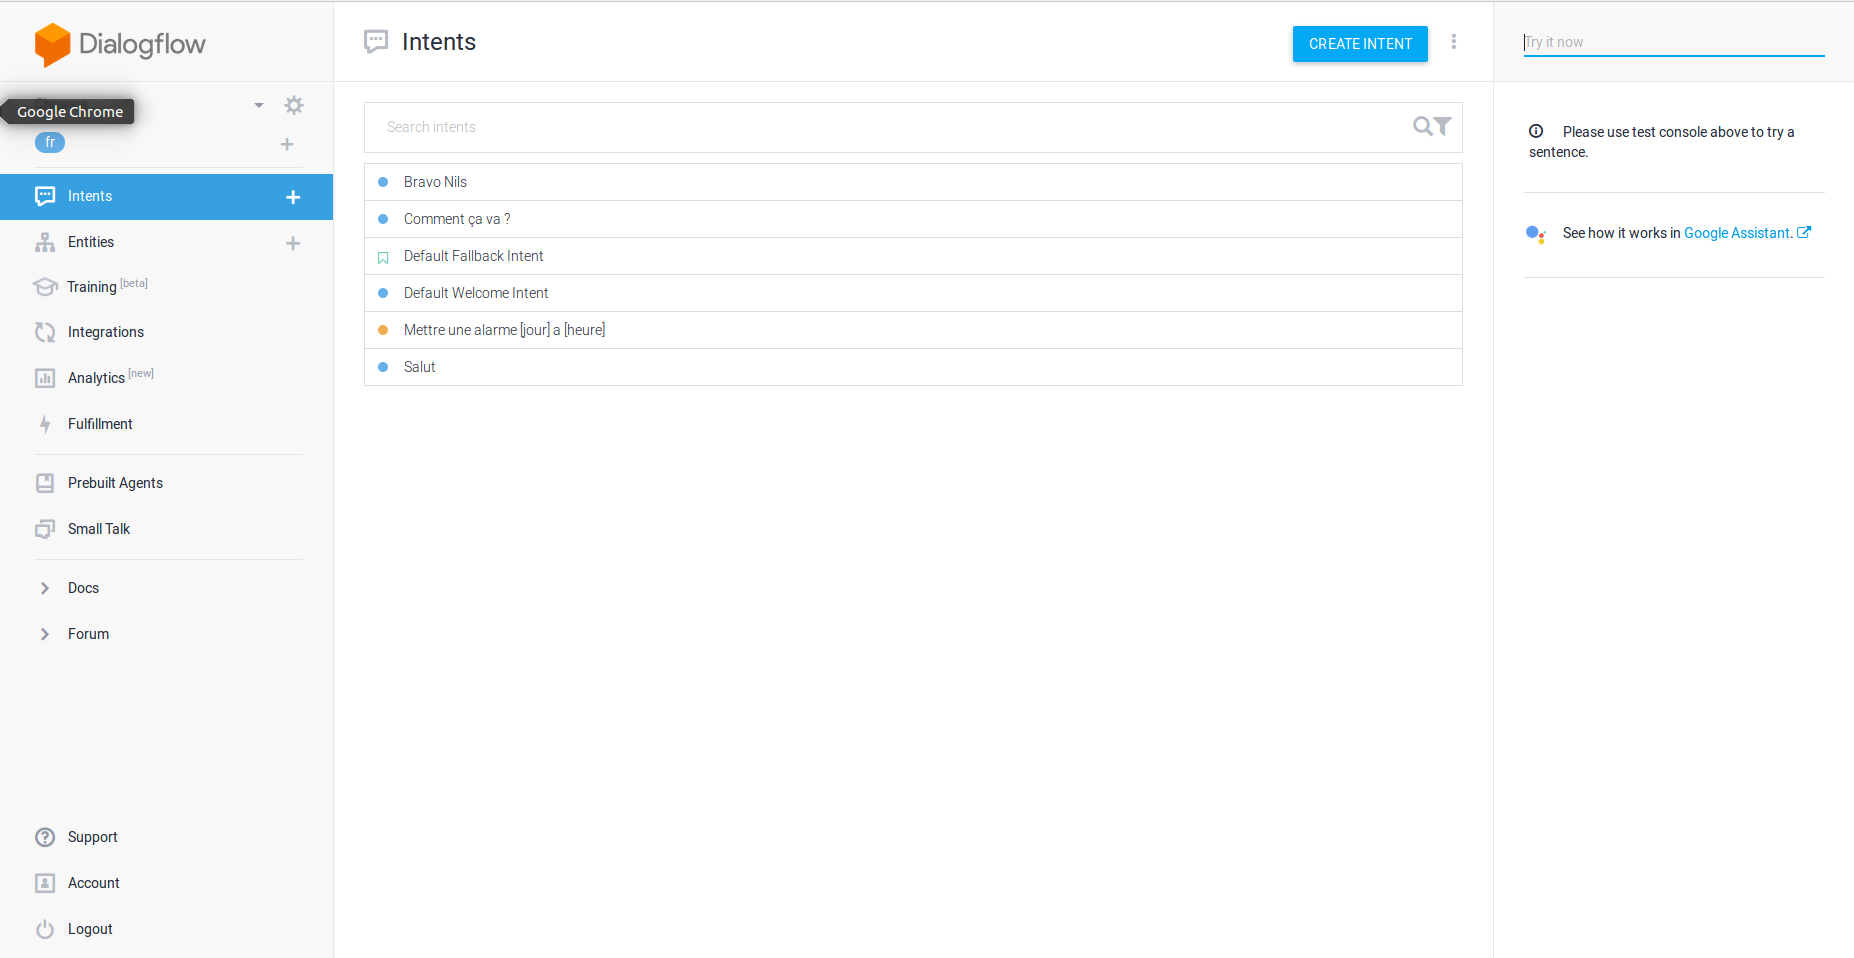
\includegraphics[width=1\textwidth]{images/dialogflow.png}
        \caption{Architecture de notre solution}
\end{figure}

Coté serveur 
    node : "MC"
    API DIalogFlow
    Interface DialogFlow 
    serveur prété par l'insa 

coté client 
    create-react-native-app - react JS 
    ejection -> react-native 
    justifier choix des librairies 

Résultats => utilisation 
    